\section{Background}

%The continuous scaling-down of
%SRAM and DRAM, which have been widely used as on-chip caches and main memories,
%is constrained by fundamental technology limits, such
%as the reduced reliability and the increases of leakage energy~\cite{ITRS07}.
%Consequently, we have seen
In recent years, significant efforts and resources have been put on
the researches and developments of emerging memory
technologies that combine attractive features
such as scalability, fast read/write, negligible
leakage, and non-volatility. Multiple promising candidates, such
as Phase-Change RAM (PCRAM) and Magnetic RAM (MRAM),
Resistive RAM (RRAM), and Memristor,
have gained substantial attentions and
are being actively pursued by industry~\cite{burr:scm08}. In this
section we will briefly describe the fundamentals of the two most promising
emerging memory technologies to be investigated in our project, namely, the Magnetic RAM (MRAM) based on Spin-Torque Transfer RAM(STT-RAM), and the Phase-Change RAM (PCRAM).

\paragraph{MRAM based on Spin-Torque Transfer RAM (STT-RAM) technology.}
STT-RAM is a new type of Magnetic RAM (MRAM)~\cite{ITRS07,Hosomi05,MRAM:TTO+06,MRAM:ZBM+06,mram:ibm:maffitt}, which
features non-volatility, fast writing/reading speed
(\textless 10ns), high programming endurance
(\textgreater 10$^{15}$cycles) and zero standby
power~\cite{ITRS07}. The storage capability or programmability of MRAM arises
from magnetic tunneling junction (MTJ), in which a thin tunneling dielectric, e.g., MgO., is sandwiched by
two ferromagnetic layers, as shown in Figure 1.
One ferromagnetic layer (``pinned layer'') is
designed to have its magnetization pinned, while the magnetization of the other layer (``free layer'')
can be flipped by a write event.
An MTJ has a low (high) resistance if the magnetizations of the free layer and the pinned layer are parallel (anti-parallel).
In first-generation MRAM design, the magnetization of free layer is changed by the
current-induced magnetic field~\cite{Motoyoshi04,Ha04}.
In STT-RAM, a new write mechanism called ``polarization-current-induced magnetization switching'' is introduced -- the magnetization of free layer is flipped by the electrical current directly.
Because the current required to switch an MTJ resistance state is
proportional to the MTJ cell area, STT-RAM is believed to have a better scaling property~\cite{Hosomi05,Kawahara07,MRAM:TTO+06}
than the first-generation MRAM.   Prototyping STT-RAM chips have been demonstrated recently by various companies and research groups~\cite{Hosomi05,Kawahara07, Nebashi09,Motoyoshi04,Andre05,Kawahara08}. Commercial MRAM products have been launched by companies like Everspin (which is a spin-off from Freescale to expedite the technology commercialization in 2008) and NEC.

\paragraph{Phase-Change RAM (PCRAM).}
PCRAM technology is based on a chalcogenide alloy (typically, Ge$_2$--Sb$_2$--Te$_5$,
GST) material, which is similar to those commonly used in optical storage means
(compact discs and digital versatile discs)~\cite{Bedeschi09}.
The data storage capability is achieved from the resistance differences between an
amorphous (high-resistance) and a crystalline (low-resistance) phase of
the chalcogenide-based material. In
SET operation, the phase change material is crystallized by
applying an electrical pulse that heats a significant portion of
the cell above its crystallization temperature. In RESET
operation, a larger electrical current is applied and then
abruptly cut off in order to melt and then quench the material, leaving it
in the amorphous state~\cite{burr:scm08}. PCRAM has shown to offer
compatible integration with CMOS technology~\cite{Oh06}, fast speed~\cite{Pirovano03},
high endurance~\cite{Lai03}, and inherent scaling of the phase-change process at 22-nm technology
node and beyond~\cite{Chen06}. Compared to STT-RAM, PCRAM is even denser with an approximate cell area of $6\sim12F^2$~\cite{ITRS07}, where F is the feature size. In addition, phase change material has a key advantage of the excellent scalability within current CMOS fabrication methodology~\cite{Cho05,Kim06,Lai01,Pirovano03,Raoux08}, with continuous density improvement~\cite{Nirshl07,Chen07-iedm,Im08}. Many PCRAM prototypes have been demonstrated in the past years by companies like Hitachi~\cite{Hanzawa07}, Samsung~\cite{Lee07-isscc}, STMicroelectronics~\cite{Bedeschi08, Sandre10}, and Numonyx~\cite{Villa10}.


%\begin{wrapfigure}{r}{0.40\textwidth}\centering \centering
%\vspace{-18pt}
%\includegraphics[width=0.40\textwidth]{./figure/MTJ.png}
%\caption{MTJ structure (a) anti-parallel, high resistance; (b) parallel, low resistance.}\label{mtj}
%\end{wrapfigure}


\paragraph{Resistive RAM (RRAM).} RRAM can generally denote all
the memory technologies that rely on the resistance change to
store the data. Based on the storage mechanisms, RRAM materials can be
cataloged as space-charge-limited-current (SCLC), filament,
programmable-metallization-cell (PMC), Schottky contact and traps (SCT), \textit{etc}.
Among them, filament-based RRAM has been wided investigated because of the potentials
on high-speed, high-endurance, and better scalability. The nsulating material between two electrodes can be made conducting
through a hopping or tunneling conduction path after the application of a sufficiently high voltage,
a process called electro-forming. The data storage could be achieved by break (``reset'') or reconnect (``set'') the conducting path.
Such switching mechanism can in fact be explained with the fourth circuit element,
i.e., the memristor or the memory resistor~\cite{Chua71,Tour08,Strukov08}. Indeed, HP Labs plan to unveil RRAM
prototype chips based on memristors with crossbar arrays soon.

%==================remove====================
\begin{comment}

\paragraph{Resistive RAM (RRAM).} RRAM can generally denote all
the memory technologies that rely on the resistance change to
store the data. From process point of view,
there are a large number of RRAM materials, including (but not limited to)
space-charge-limited-current (SCLC), filament,
programmable-metallization-cell (PMC), Schottky contact and traps
(SCT), \textit{etc}. From design point of view, R-RAM technologies
can be cataloged into only two operation types: unipolar switching
and bipolar switching. Unipolar operation executes the
programming/erasing by using short and long pulse, or by using
high and low voltage with the same voltage polarity, while bipolar
operation is achieved by short pulses with opposite voltage
polarity.

Filament-based R-RAM is a typical example of unipolar
switching~\cite{Inoue}. A filament or conducting path is formed in
an insulating dielectric by applying a sufficiently high voltage.
Once the filament is formed, it can be SET (leading to a
low-resistance) or RESET (leading to a high-resistance) with
appropriate voltages. PMC~\cite{Kozicki05} is a promising bipolar
switching technology, which is composed of two solid metal
electordes -- relatively, one is inert and the other is
electrochemically active. Between the two electrodes locates a
thin electrolyte film. When a negative bias is applied to the
inert electrode in programming operation, metal ions in the
electrolyte together with those flew from the positive active
electrode can be reduced by the inert electrode. As a result, the
metal ions form a small metallic ``nanowire'' between the two
electrodes, which produces a low resistance. In erasing operation,
a positive bias is applied on the inert electrode. metal ions
migrate back into the electrolyte and eventually to the
negatively-charged active electrode. The ``nanowire'' is broken
and the resistance increase back.

RRAM has the characteristics of non-volatility, high-speed,
high-endurance, zero standby power. Potentially it can achieve the
smallest memory cell size -- 4F$^2$. Furthermore, the integration
of RRAM supports cross-point structure, which can further improve
memory density (See section~\ref{C2.3-RRAM}). Hence, RRAM is
expected to be the candidate of main storage in near
future~\cite{ITRS-ROADMAP-reference}.
\end{comment}

\begin{figure}
%\begin{wrapfigure}{r}{0.6\textwidth}\centering
\centering
\vspace{-10pt} 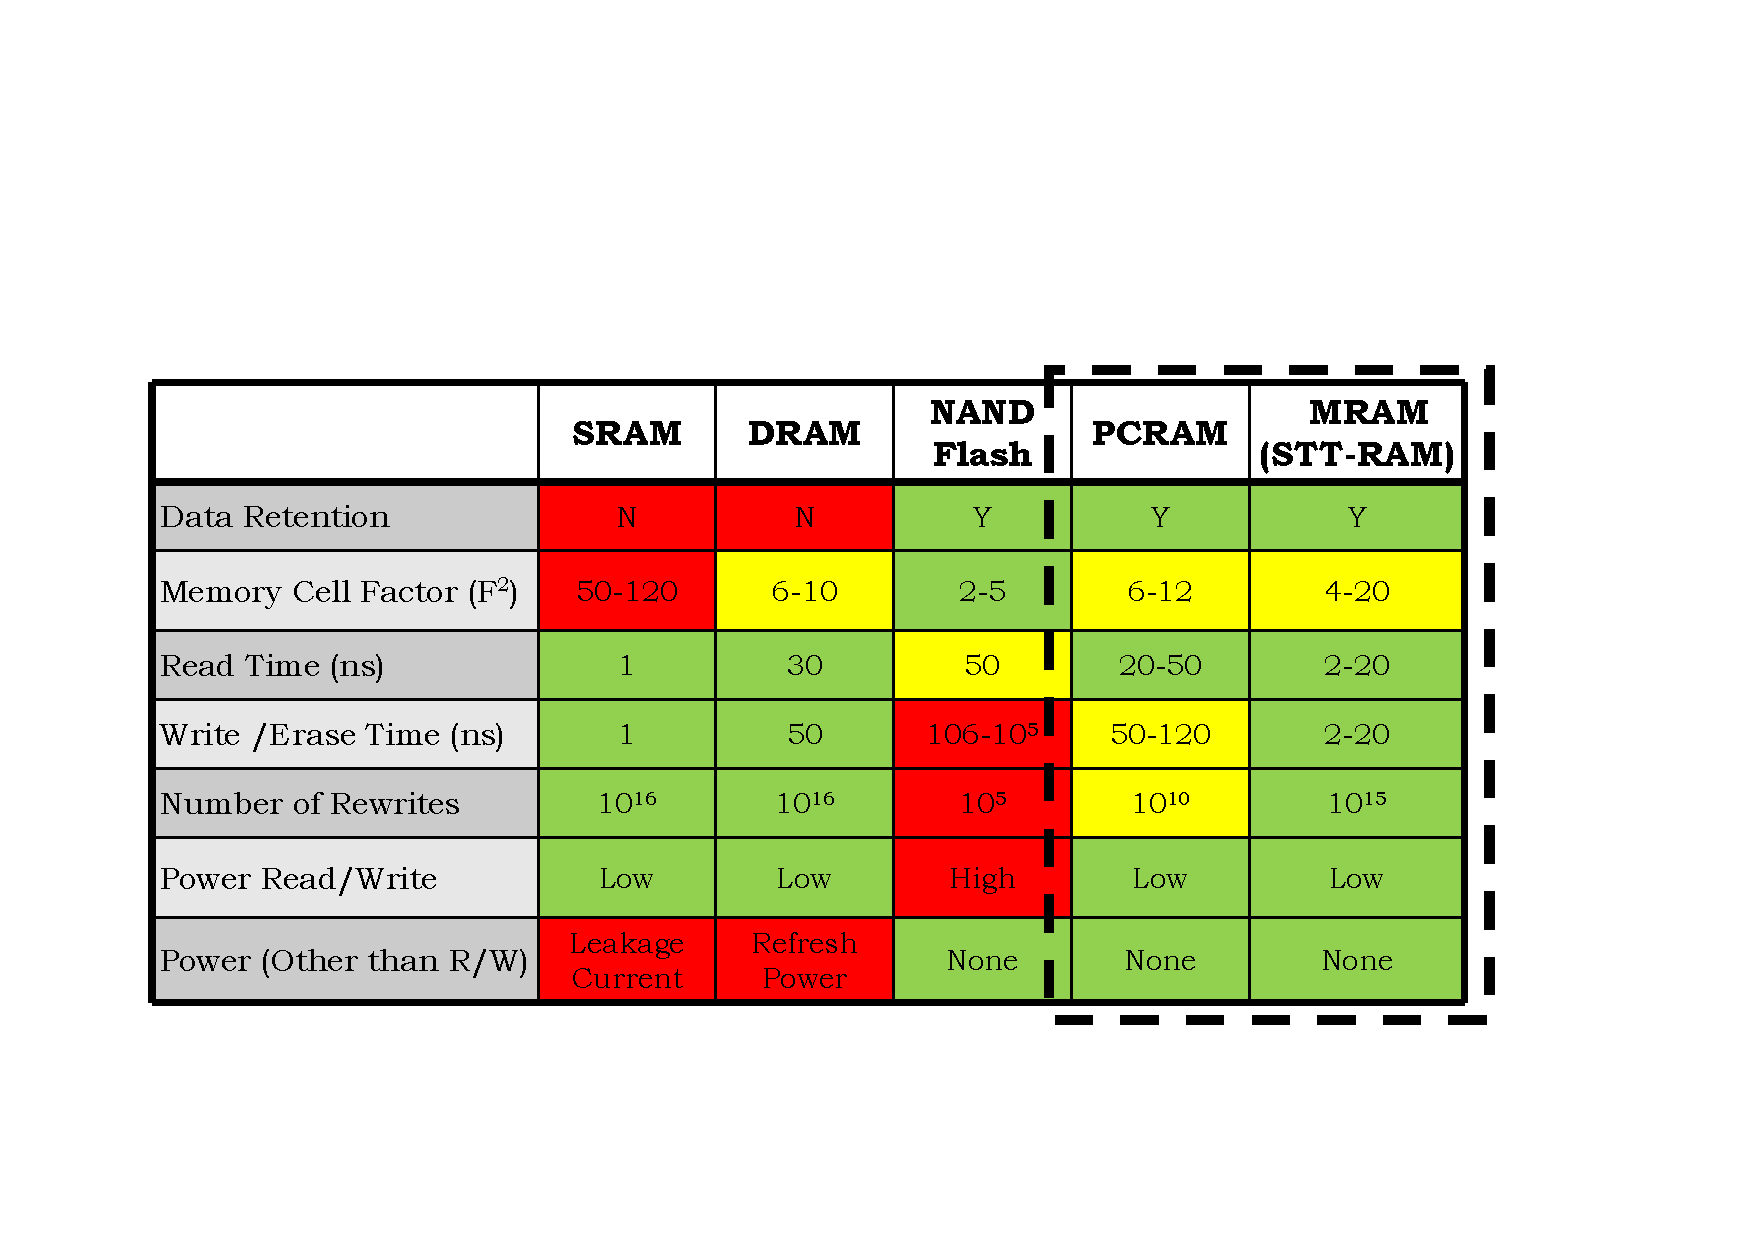
\includegraphics[width=0.7\textwidth]{./figure/table.pdf} \vspace{-10pt}
\caption{The comparison of various memory
technologies~\cite{ITRS07}.}\label{table} \vspace{-10pt}
%\end{wrapfigure}
\end{figure}
\paragraph{Summary.} Figure~\ref{table} illustrates the comparison of
two emerging memory technologies -- PCRAM and MRAM (STT-RAM)  --
against the traditional main-stream SRAM, DRAM, and NAND-based Flash memory~\cite{ITRS07}.
Note that both CMOS-compatible embedded MRAM (NEC)~\cite{MRAM:NEC09} and embedded PCRAM (Hitachi and STMicro)~\cite{PRAM:Hitachi2007,PRAM:ST2004} have been demonstrated, paving the way of integrating
these NVMs to the traditional memory hierarchies. In addition, the emerging 3D integration technologies~\cite{xie:jetcs06,Xie:dac08}
enables cost-effective integration of these NVMs with CMOS logic circuits. With all the NVM technology advances in recent years, it is anticipated that the emerging NVM technologies will break important ground and move closer to market in the near future (``Non-volatile memory goes commercial", EEtimes, 12/02/2009).


\begin{comment}
\paragraph{Memristor.} Memristor -- the fourth fundamental passive circuit
element -- was predicted by Professor Chua in 1971~\cite{Chua71},
based on the completeness of circuit theory (See
Figure~\ref{memristor}). Different from other electrical
parameters resistance (\textit{R}), capacitance (\textit{C}) and
inductance (\textit{L}), memristance (\textit{M}) is a function of
charge (\textit{q}),  which depends upon the historic behavior of
the current (or voltage) profile~\cite{Chua76}.

%\begin{figure}
%\includegraphics[width=0.40\textwidth]{./figure/HL-memristor.eps}
%caption{Four fundamental passive circuit
%elements.}\label{memristor}
%\end{figure}

In 2008, 37 years after memristor was predicted in theory, the
researchers at HP reported the first real device of a memristor.
The memristive effect was achieved in a solid-state thin film
two-terminal device by moving the doping front along the
device~\cite{Tour08}. Afterwards, magnetic technology provides the
other possible methods to build a memristive
system~\cite{Pershin08,Wang09}. Due to its unique historic
characteristic, memristor has very broad application including
nonvolatile memory, signal processing, control and learning system
etc~\cite{Chen09}.
\end{comment}
